\section{逼真相机}\label{sec:逼真相机}
\begin{remark}
    本节含有高级内容,第一次阅读时可以跳过。
\end{remark}

薄透镜模型使得能渲染因景深而模糊的图像,
但它只是对多个\keyindex{透镜元件}{lens element}{}构成的
真实相机透镜系统非常粗糙的近似,而每个透镜元件都会改变穿过它的辐射分布
(\reffig{6.15}展示了具有8个元件的22mm焦距\keyindex{广角}{wide-angle}{}镜头横截面)。
即使基本的手机相机也趋于有五个左右独立的透镜元件,
而\keyindex{数码单镜头反光相机}{digital single-lens reflex camera}{camera相机}
(数码单反相机,DSLR)镜头可能有十个或更多。
通常,具备更大数量透镜元件的更复杂透镜系统能
比更简单的透镜系统创建更高质量的图像。
\begin{figure}[htbp]
    \centering%LaTeX with PSTricks extensions
%%Creator: Inkscape 1.1.1 (3bf5ae0d25, 2021-09-20)
%%Please note this file requires PSTricks extensions
\psset{xunit=.5pt,yunit=.5pt,runit=.5pt}
\begin{pspicture}(480,210.66666667)
{
\newrgbcolor{curcolor}{0 0 0}
\pscustom[linewidth=1.33333333,linecolor=curcolor]
{
\newpath
\moveto(102.07812533,200.869792)
\curveto(80.78645867,139.869792)(80.78645867,73.46354133)(102.07812533,12.46354133)
}
}
{
\newrgbcolor{curcolor}{0 0 0}
\pscustom[linewidth=1.33333333,linecolor=curcolor]
{
\newpath
\moveto(102.125,200.34895867)
\lineto(129.375,200.34895867)
}
}
{
\newrgbcolor{curcolor}{0 0 0}
\pscustom[linewidth=1.33333333,linecolor=curcolor]
{
\newpath
\moveto(102.125,11.942708)
\lineto(129.375,11.942708)
}
}
{
\newrgbcolor{curcolor}{0 0 0}
\pscustom[linewidth=1.33333333,linecolor=curcolor]
{
\newpath
\moveto(129.375,200.34895867)
\lineto(129.375,177.625)
}
}
{
\newrgbcolor{curcolor}{0 0 0}
\pscustom[linewidth=1.33333333,linecolor=curcolor]
{
\newpath
\moveto(129.375,11.942708)
\lineto(129.375,34.66145867)
}
}
{
\newrgbcolor{curcolor}{0 0 0}
\pscustom[linewidth=1.33333333,linecolor=curcolor]
{
\newpath
\moveto(129.95833333,178.14583333)
\curveto(108.70312533,160.494792)(96.41145867,134.29687467)(96.41145867,106.66666667)
\curveto(96.41145867,79.03645867)(108.70312533,52.83854133)(129.95833333,35.1875)
}
}
{
\newrgbcolor{curcolor}{0 0 0}
\pscustom[linewidth=1.33333333,linecolor=curcolor]
{
\newpath
\moveto(187.03125067,155.77604133)
\curveto(170.58854133,125.09895867)(170.58854133,88.23437467)(187.03125067,57.557292)
}
}
{
\newrgbcolor{curcolor}{0 0 0}
\pscustom[linewidth=1.33333333,linecolor=curcolor]
{
\newpath
\moveto(187.5625,155.255208)
\lineto(211.682292,155.255208)
}
}
{
\newrgbcolor{curcolor}{0 0 0}
\pscustom[linewidth=1.33333333,linecolor=curcolor]
{
\newpath
\moveto(187.5625,57.03125067)
\lineto(211.682292,57.03125067)
}
}
{
\newrgbcolor{curcolor}{0 0 0}
\pscustom[linewidth=1.33333333,linecolor=curcolor]
{
\newpath
\moveto(211.682292,155.255208)
\lineto(211.682292,145.119792)
}
}
{
\newrgbcolor{curcolor}{0 0 0}
\pscustom[linewidth=1.33333333,linecolor=curcolor]
{
\newpath
\moveto(211.682292,57.03125067)
\lineto(211.682292,67.17187467)
}
}
{
\newrgbcolor{curcolor}{0 0 0}
\pscustom[linewidth=1.33333333,linecolor=curcolor]
{
\newpath
\moveto(211.52604133,67.692708)
\curveto(217.22916667,93.364584)(217.22916667,119.96874933)(211.52604133,145.64062533)
}
}
{
\newrgbcolor{curcolor}{0 0 0}
\pscustom[linewidth=1.33333333,linecolor=curcolor]
{
\newpath
\moveto(211.682292,145.119792)
\lineto(231.1875,145.119792)
}
}
{
\newrgbcolor{curcolor}{0 0 0}
\pscustom[linewidth=1.33333333,linecolor=curcolor]
{
\newpath
\moveto(211.682292,67.17187467)
\lineto(231.1875,67.17187467)
}
}
{
\newrgbcolor{curcolor}{0 0 0}
\pscustom[linewidth=1.33333333,linecolor=curcolor]
{
\newpath
\moveto(231.1875,145.119792)
\lineto(231.1875,142.5)
}
}
{
\newrgbcolor{curcolor}{0 0 0}
\pscustom[linewidth=1.33333333,linecolor=curcolor]
{
\newpath
\moveto(231.1875,67.17187467)
\lineto(231.1875,69.79166667)
}
}
{
\newrgbcolor{curcolor}{0 0 0}
\pscustom[linewidth=1.33333333,linecolor=curcolor]
{
\newpath
\moveto(231.33333333,143.02083333)
\curveto(229.77083333,118.807292)(229.77083333,94.52604133)(231.33333333,70.3125)
}
}
{
\newrgbcolor{curcolor}{0 0 0}
\pscustom[linewidth=2.66666667,linecolor=curcolor]
{
\newpath
\moveto(236.510416,140.92708267)
\lineto(236.510416,175.70312533)
}
}
{
\newrgbcolor{curcolor}{0 0 0}
\pscustom[linewidth=2.66666667,linecolor=curcolor]
{
\newpath
\moveto(236.510416,71.364584)
\lineto(236.510416,36.58333333)
}
}
{
\newrgbcolor{curcolor}{0 0 0}
\pscustom[linewidth=1.33333333,linecolor=curcolor]
{
\newpath
\moveto(247.53125067,74.15625067)
\curveto(257.25,94.739584)(257.25,118.59374933)(247.53125067,139.17708267)
}
}
{
\newrgbcolor{curcolor}{0 0 0}
\pscustom[linewidth=1.33333333,linecolor=curcolor]
{
\newpath
\moveto(247.32291733,142.5)
\lineto(266.23437467,142.5)
}
}
{
\newrgbcolor{curcolor}{0 0 0}
\pscustom[linewidth=1.33333333,linecolor=curcolor]
{
\newpath
\moveto(247.32291733,69.79166667)
\lineto(266.23437467,69.79166667)
}
}
{
\newrgbcolor{curcolor}{0 0 0}
\pscustom[linewidth=1.33333333,linecolor=curcolor]
{
\newpath
\moveto(247.32291733,142.5)
\lineto(247.32291733,138.65104133)
}
}
{
\newrgbcolor{curcolor}{0 0 0}
\pscustom[linewidth=1.33333333,linecolor=curcolor]
{
\newpath
\moveto(247.32291733,69.79166667)
\lineto(247.32291733,73.635416)
}
}
{
\newrgbcolor{curcolor}{0 0 0}
\pscustom[linewidth=1.33333333,linecolor=curcolor]
{
\newpath
\moveto(265.98437467,70.3125)
\curveto(276.25,93.46354133)(276.25,119.869792)(265.98437467,143.02083333)
}
}
{
\newrgbcolor{curcolor}{0 0 0}
\pscustom[linewidth=1.33333333,linecolor=curcolor]
{
\newpath
\moveto(273.57812533,64.369792)
\curveto(274.47916667,92.5625)(274.47916667,120.77083333)(273.57812533,148.96354133)
}
}
{
\newrgbcolor{curcolor}{0 0 0}
\pscustom[linewidth=1.33333333,linecolor=curcolor]
{
\newpath
\moveto(274.17187467,151.58854133)
\lineto(278.78125067,151.58854133)
}
}
{
\newrgbcolor{curcolor}{0 0 0}
\pscustom[linewidth=1.33333333,linecolor=curcolor]
{
\newpath
\moveto(274.17187467,60.70312533)
\lineto(278.78125067,60.70312533)
}
}
{
\newrgbcolor{curcolor}{0 0 0}
\pscustom[linewidth=1.33333333,linecolor=curcolor]
{
\newpath
\moveto(274.17187467,151.58854133)
\lineto(274.17187467,148.442708)
}
}
{
\newrgbcolor{curcolor}{0 0 0}
\pscustom[linewidth=1.33333333,linecolor=curcolor]
{
\newpath
\moveto(274.17187467,60.70312533)
\lineto(274.17187467,63.84895867)
}
}
{
\newrgbcolor{curcolor}{0 0 0}
\pscustom[linewidth=1.33333333,linecolor=curcolor]
{
\newpath
\moveto(278.3125,61.22395867)
\curveto(291.4375,72.67708267)(298.97395867,89.244792)(298.97395867,106.66666667)
\curveto(298.97395867,124.08854133)(291.4375,140.65625067)(278.3125,152.10937467)
}
}
{
\newrgbcolor{curcolor}{0 0 0}
\pscustom[linewidth=1.33333333,linecolor=curcolor]
{
\newpath
\moveto(278.78125067,154.90625067)
\lineto(300.739584,154.90625067)
}
}
{
\newrgbcolor{curcolor}{0 0 0}
\pscustom[linewidth=1.33333333,linecolor=curcolor]
{
\newpath
\moveto(278.78125067,57.385416)
\lineto(300.739584,57.385416)
}
}
{
\newrgbcolor{curcolor}{0 0 0}
\pscustom[linewidth=1.33333333,linecolor=curcolor]
{
\newpath
\moveto(278.78125067,154.90625067)
\lineto(278.78125067,151.58854133)
}
}
{
\newrgbcolor{curcolor}{0 0 0}
\pscustom[linewidth=1.33333333,linecolor=curcolor]
{
\newpath
\moveto(278.78125067,57.385416)
\lineto(278.78125067,60.70312533)
}
}
{
\newrgbcolor{curcolor}{0 0 0}
\pscustom[linewidth=1.33333333,linecolor=curcolor]
{
\newpath
\moveto(301.28125067,57.90625067)
\curveto(313.60937467,89.244792)(313.60937467,124.08854133)(301.28125067,155.42708267)
}
}
{
\newrgbcolor{curcolor}{0 0 0}
\pscustom[linewidth=1.33333333,linecolor=curcolor]
{
\newpath
\moveto(310.05208267,53.35937467)
\curveto(329.29166667,64.20833333)(341.192708,84.57812533)(341.192708,106.66666667)
\curveto(341.192708,128.755208)(329.29166667,149.125)(310.05208267,159.97395867)
}
}
{
\newrgbcolor{curcolor}{0 0 0}
\pscustom[linewidth=1.33333333,linecolor=curcolor]
{
\newpath
\moveto(310.46354133,177.625)
\lineto(318.90104133,177.625)
}
}
{
\newrgbcolor{curcolor}{0 0 0}
\pscustom[linewidth=1.33333333,linecolor=curcolor]
{
\newpath
\moveto(310.46354133,34.66145867)
\lineto(318.90104133,34.66145867)
}
}
{
\newrgbcolor{curcolor}{0 0 0}
\pscustom[linewidth=1.33333333,linecolor=curcolor]
{
\newpath
\moveto(310.46354133,177.625)
\lineto(310.46354133,159.45312533)
}
}
{
\newrgbcolor{curcolor}{0 0 0}
\pscustom[linewidth=1.33333333,linecolor=curcolor]
{
\newpath
\moveto(310.46354133,34.66145867)
\lineto(310.46354133,52.83854133)
}
}
{
\newrgbcolor{curcolor}{0 0 0}
\pscustom[linewidth=1.33333333,linecolor=curcolor]
{
\newpath
\moveto(318.75,35.1875)
\curveto(339.32291733,53.244792)(351.114584,79.29166667)(351.114584,106.66666667)
\curveto(351.114584,134.04166667)(339.32291733,160.08854133)(318.75,178.14583333)
}
}
{
\newrgbcolor{curcolor}{0 0 0}
\pscustom[linewidth=1.33333333,linecolor=curcolor]
{
\newpath
\moveto(469.09374933,10.8125)
\lineto(469.09374933,201.47395867)
}
}
{
\newrgbcolor{curcolor}{0 0 0}
\pscustom[linewidth=1.33333333,linecolor=curcolor]
{
\newpath
\moveto(469.09374933,106.14583333)
\lineto(9.57291733,106.14583333)
}
}
\end{pspicture}

    \caption{广角透镜系统的横截面(在pbrt发行版的{\ttfamily scenes/lenses/wide.22mm.dat}
    中)。透镜坐标系统让胶片平面垂直于$z$轴且位于$z=0$处。
    透镜在左边负z轴上,然后场景在透镜左侧。透镜系统中部表示为粗黑线的光圈阻挡命中它的光线。
    在许多透镜系统中,可以调整光圈大小以在更短曝光时间(大光圈)和更大景深(小光圈)间权衡。}
    \label{fig:6.15}
\end{figure}

本节讨论\refvar{RealisticCamera}{}的实现,
它模拟光穿过像\reffig{6.15}那样的透镜系统后聚焦并渲染像\reffig{6.16}那样的图像。
其实现基于光线追踪,即相机追随光路穿过透镜元件,
并考虑具有不同折射率的介质(空气,各类玻璃)间界面的折射,
直到光路要么退出光学系统要么被光圈或镜头罩吸收。
离开前端镜头元件的光线代表相机响应曲线,可用于估计
沿任意光线入射辐亮度的积分器,例如\refvar{SamplerIntegrator}{}。
\refvar{RealisticCamera}{}的实现在文件\href{https://github.com/mmp/pbrt-v3/tree/master/src/cameras/realistic.h}{\ttfamily cameras/realistic.h}
和\href{https://github.com/mmp/pbrt-v3/tree/master/src/cameras/realistic.cpp}{\ttfamily cameras/realistic.cpp}中。
\begin{figure}[htbp]
    \centering\includegraphics[width=0.6\linewidth]{chap06/sanmiguel-fisheye.png}
    \caption{用鱼眼透镜和很宽视场渲染的图像。注意边缘暗处是
        准确模拟成像辐射度量(\refsub{相机测量方程})所致,
        而直线扭曲为曲线则是许多广角镜头的特点,但在用投影矩阵表示透镜投影模型时没有考虑。}
    \label{fig:6.16}
\end{figure}
\begin{lstlisting}
`\initcode{RealisticCamera Declarations}{=}`
class `\initvar{RealisticCamera}{}` : public `\refvar{Camera}{}` {
public:
    `\refcode{RealisticCamera Public Methods}{}`
private:
    `\refcode{RealisticCamera Private Declarations}{}`
    `\refcode{RealisticCamera Private Data}{}`
    `\refcode{RealisticCamera Private Methods}{}`
};
\end{lstlisting}

除了把相机放置于场景中的常见变换、\refvar{Film}{}以及快门打开和关闭的时间外,
\refvar{RealisticCamera}{}构造函数还接收透镜系统描述文件的文件名、
到期望的焦平面的距离以及光圈直径。之后有了第\refchap{蒙特卡洛积分}蒙特卡洛积分与
\refsub{相机测量方程}成像辐射度量的预备知识后,
将在\refsub{采样相机1}介绍参数{\ttfamily simpleWeighting}的作用。
\begin{lstlisting}
`\initcode{RealisticCamera Method Definitions}{=}\initnext{RealisticCameraMethodDefinitions}`
`\refvar{RealisticCamera}{}`::`\refvar{RealisticCamera}{}`(const `\refvar{AnimatedTransform}{}` &CameraToWorld,
        `\refvar{Float}{}` shutterOpen, `\refvar{Float}{}` shutterClose, `\refvar{Float}{}` apertureDiameter,
        `\refvar{Float}{}` focusDistance, bool simpleWeighting, const char *lensFile,
        `\refvar{Film}{}` *film, const `\refvar{Medium}{}` *medium)
    : `\refvar{Camera}{}`(CameraToWorld, shutterOpen, shutterClose, film, medium),
      simpleWeighting(simpleWeighting) {
    `\refcode{Load element data from lens description file}{}`
    `\refcode{Compute lens–film distance for given focus distance}{}`
    `\refcode{Compute exit pupil bounds at sampled points on the film}{}`
}
\end{lstlisting}
\begin{lstlisting}
`\initcode{Load element data from lens description file}{=}`
std::vector<`\refvar{Float}{}`> lensData;
if (ReadFloatFile(lensFile, &lensData) == false) {
    `\refvar{Error}{}`("Error reading lens specification file \"%s\".", lensFile);
    return;
}
if ((lensData.size() % 4) != 0) {
    `\refvar{Error}{}`("Excess values in lens specification file \"%s\"; "
          "must be multiple-of-four values, read %d.",
          lensFile, (int)lensData.size());
    return;
}
for (int i = 0; i < (int)lensData.size(); i += 4) {
    if (lensData[i] == 0) {
        if (apertureDiameter > lensData[i+3]) {
            `\refvar{Warning}{}`("Specified aperture diameter %f is greater than maximum "
                    "possible %f.  Clamping it.", apertureDiameter, lensData[i+3]);
        } else {
            lensData[i+3] = apertureDiameter;
        }
    }
    `\refvar{elementInterfaces}{}`.push_back((`\refvar{LensElementInterface}{}`)
        {lensData[i] * (`\refvar{Float}{}`).001, lensData[i+1] * (`\refvar{Float}{}`).001, lensData[i+2],
         lensData[i+3] * `\refvar{Float}{}`(.001) / `\refvar{Float}{}`(2.)});
}
\end{lstlisting}
\begin{lstlisting}
`\initcode{RealisticCamera Private Data}{=}\initnext{RealisticCameraPrivateData}`
const bool `\initvar{simpleWeighting}{}`;
\end{lstlisting}

在从磁盘加载透镜描述文件之后,构造函数调整透镜与
胶片间的距离使得焦平面位于期望的深度即{\ttfamily focusDistance},
然后预先计算一些关于离胶片最近透镜元件的哪部分面积让光从场景射到胶片的信息,
就像在胶片平面上各点看到的那样。在介绍完背景材料之后,
\refsub{对焦}和\refsub{出射瞳}将分别定义代码片
\refcode{Compute lens-film distance for given focus distance}{}
和\refcode{Compute exit pupil bounds at sampled points on the film}{}。

\subsection{透镜系统表示}\label{sub:透镜系统表示}
透镜系统由一系列透镜元件组成,每个元件通常是某种形制的玻璃。
透镜系统设计者的挑战是在有限空间、成本和生产难度下
设计一组能在胶片或传感器上高质量成像的元件
(例如为了让保持手机变薄,其相机厚度非常有限)。

最容易生产的是横截面为球形的透镜,
透镜系统通常是绕\keyindex{光轴}{optical axis}{}对称的,习惯记为$z$。
我们将假设这两个性质在本节下文中成立。
用胶片对齐到平面$z=0$且透镜在胶片左侧沿$-z$轴放置的坐标系统定义透镜系统。

透镜系统常表示为独立透镜元件(或空气)间的一系列界面,
而不是每个元件的显式表示。\reftab{6.1}展示了定义每个界面的量。
表中最后一项定义了最右边的界面,如\reffig{6.17}所示:
它是个半径等于曲率半径的球体块。元件的厚度是沿$z$到右边下一个
元件(或胶片平面)的距离,\keyindex{折射率}{index of refraction}{}是
对界面右边的介质而言的。元件在$z$轴上下的范围由光圈直径设置。
\begin{table}[htbp]
    \centering
    \begin{tabular}{SSSS}
        \toprule
        \ \ \ \textbf{曲率半径} & \ \ \ \ \textbf{厚度} & \ \textbf{折射率} & \textbf{光圈直径} \\
        \midrule
        35.98738                & 1.21638               & 1.54              & 23.716            \\
        11.69718                & 9.9957                & 1                 & 17.996            \\
        13.08714                & 5.12622               & 1.772             & 12.364            \\
        -22.63294               & 1.76924               & 1.617             & 9.812             \\
        71.05802                & 0.8184                & 1                 & 9.152             \\
        0                       & 2.27766               & 0                 & 8.756             \\
        -9.58584                & 2.43254               & 1.617             & 8.184             \\
        -11.28864               & 0.11506               & 1                 & 9.152             \\
        -166.7765               & 3.09606               & 1.713             & 10.648            \\
        -7.5911                 & 1.32682               & 1.805             & 11.44             \\
        -16.7662                & 3.98068               & 1                 & 12.276            \\
        -7.70286                & 1.21638               & 1.617             & 13.42             \\
        -11.97328               & (取决于焦点)        & 1                 & 17.996            \\
        \bottomrule
    \end{tabular}
    \caption{\reffig{6.15}中透镜系统的表格化描述。每行描述了两个透镜元件间的界面、
        元件与空气间的界面或者光圈。第一行描述了最左边的界面。半径为0的元件对应光圈。
        距离单位为mm。}
    \label{tab:6.1}
\end{table}
\begin{figure}[htbp]
    \centering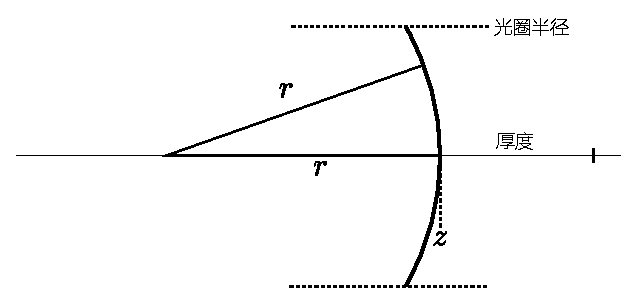
\includegraphics[width=0.6\linewidth]{chap06/Lenselement.eps}
    \caption{透镜界面(实曲线)与光轴相交于位置$z$。界面几何形状由
        表示其在光轴上下方范围的光圈半径以及元件的曲率半径$r$描述。
        如果元件有球形横截面,则它的轮廓由球心在光轴上距离$r$的球体给定,
        该球体也穿过$z$。如果$r$是负的,则元件界面就如从场景中看到那样是凹的
        (如图所示);否则就是\protect\keyindex{凸}{convex}{}的。透镜厚度给出了到
        右边下一个界面的距离,或者对于最右边的界面是到胶片平面的距离。}
    \label{fig:6.17}
\end{figure}

结构体\refvar{LensElementInterface}{}表示单个透镜元件界面。
\begin{lstlisting}
`\initcode{RealisticCamera Private Declarations}{=}`
struct `\initvar{LensElementInterface}{}` {
    `\refvar{Float}{}` `\initvar{curvatureRadius}{}`;
    `\refvar{Float}{}` `\initvar{thickness}{}`;
    `\refvar{Float}{}` `\initvar[LensElementInterface::eta]{eta}{}`;
    `\refvar{Float}{}` `\initvar{apertureRadius}{}`;
};
\end{lstlisting}

这里没有介绍的代码片\refcode{Load element data from lens description file}{}
\sidenote{译者注:我补充回来了。}读取透镜元件
并初始化数组\refvar[elementInterfaces]{RealisticCamera::elementInterfaces}{}。
见源代码中的注释了解该文件格式的细节,它并行化\reftab{6.1}中的结构,
并见pbrt发行版中的目录{\ttfamily scenes/lenses}了解大量透镜描述示例。

对从文件读取的值做了两个调整:第一,透镜系统传统上用毫米单位描述,
但pbrt假设场景单位用米。因此,除了折射率外的域都按1/1000缩小。
第二,元件直径被除以二;在下面的代码中半径是用起来更方便的量。
\begin{lstlisting}
`\refcode{RealisticCamera Private Data}{+=}\lastnext{RealisticCameraPrivateData}`
std::vector<`\refvar{LensElementInterface}{}`> `\initvar{elementInterfaces}{}`;
\end{lstlisting}

一旦加载完透镜界面描述,让一些关于透镜系统的值随时可得是很有用的。
\refvar{LensRearZ}{()}和\refvar{LensFrontZ}{()}分别返回
透镜系统尾部和头部元件的$z$深度。注意返回的$z$深度在相机空间中,
而不是透镜空间中,所以为正值。
\begin{lstlisting}
`\initcode{RealisticCamera Private Methods}{=}\initnext{RealisticCameraPrivateMethods}`
`\refvar{Float}{}` `\initvar{LensRearZ}{}`() const {
    return `\refvar{elementInterfaces}{}`.back().`\refvar{thickness}{}`;
}
\end{lstlisting}

求头部元件$z$位置需要求所有元件厚度之和(见\reffig{6.18})。
任何位于系统性能敏感部分的代码都不需要该值,
所以在需要时重算它就行。如果该方法对性能有影响,
最好还是在\refvar{RealisticCamera}{}中缓存该值。
\begin{figure}[htbp]
    \centering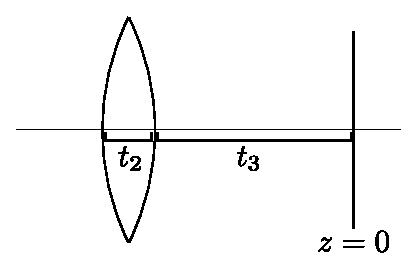
\includegraphics[width=0.4\linewidth]{chap06/Elementthicknessandposition.eps}
    \caption{元件厚度与光轴上位置的关系。胶片平面位于$z=0$,尾部元件的厚度$t_3$给出
        了从胶片到其界面的距离;这里尾部界面与轴交于$z=-t_3$。下一个元件厚度为$t_2$且
        位于$z=-t_3-t_2$,以此类推。头部元件交$z$轴于$\sum_i-t_i$。}
    \label{fig:6.18}
\end{figure}
\begin{lstlisting}
`\refcode{RealisticCamera Private Methods}{+=}\lastnext{RealisticCameraPrivateMethods}`
`\refvar{Float}{}` `\initvar{LensFrontZ}{}`() const {
    `\refvar{Float}{}` zSum = 0;
    for (const `\refvar{LensElementInterface}{}` &element : `\refvar{elementInterfaces}{}`)
        zSum += element.`\refvar{thickness}{}`;
    return zSum;
}
\end{lstlisting}

\refvar{RearElementRadius}{()}按单位米返回尾部元件光圈半径。
\begin{lstlisting}
`\refcode{RealisticCamera Private Methods}{+=}\lastnext{RealisticCameraPrivateMethods}`
`\refvar{Float}{}` `\initvar{RearElementRadius}{}`() const {
    return `\refvar{elementInterfaces}{}`.back().`\refvar{apertureRadius}{}`;
}
\end{lstlisting}
\subsection{追踪穿过透镜的光线}\label{sub:追踪穿过透镜的光线}

\subsection{厚透镜近似}\label{sub:厚透镜近似}
\subsection{对焦}\label{sub:对焦}
\subsection{出射瞳}\label{sub:出射瞳}
\subsection{相机测量方程}\label{sub:相机测量方程}